\chapter{Conclusion}
\section{General conclusions}
The usage of Computer Vision and its algorithms to process images is
still something new and not so extended. Nevertheless, its potential is
so high. Starting with low knowledges in the area, this project is an
example of the versatility of this techniques to specific cases in
the real world. There are still too much to investigate in this branch
of the Computer Science, and we are proud of take a part in a project
with this characteristics.\\
When people talk about Computer Vision maybe they tend to think,
innocently, that it is a specific area of Computer Science. However
it goes further, because its funcionalities can be applied to each
type of image, which in this case have been \emph{tomographies}.
The results of processing them are so satisfactories, for us and
for the medical team that collaborated with us in the project, 
providing technical knowledge in the area and images to study.

\section{Conclusions about pores detection in the papilla}
The detection of pores in the optical papilla has been succeded thanks
to, in part, SimpleCV library and its functionalities to detect 
\emph{blobs}. It has achieve a negligible time of processing comparing
it to the time spended by medical staff to mark them. Also their 
measurement is still more exact than the estimation they were doing
until now. \\
The next images show and example:

    \begin{figure}[H]
      \caption{Original Image}
      \centering \setlength\fboxsep{0pt} \setlength\fboxrule{0.5pt}
      \fbox{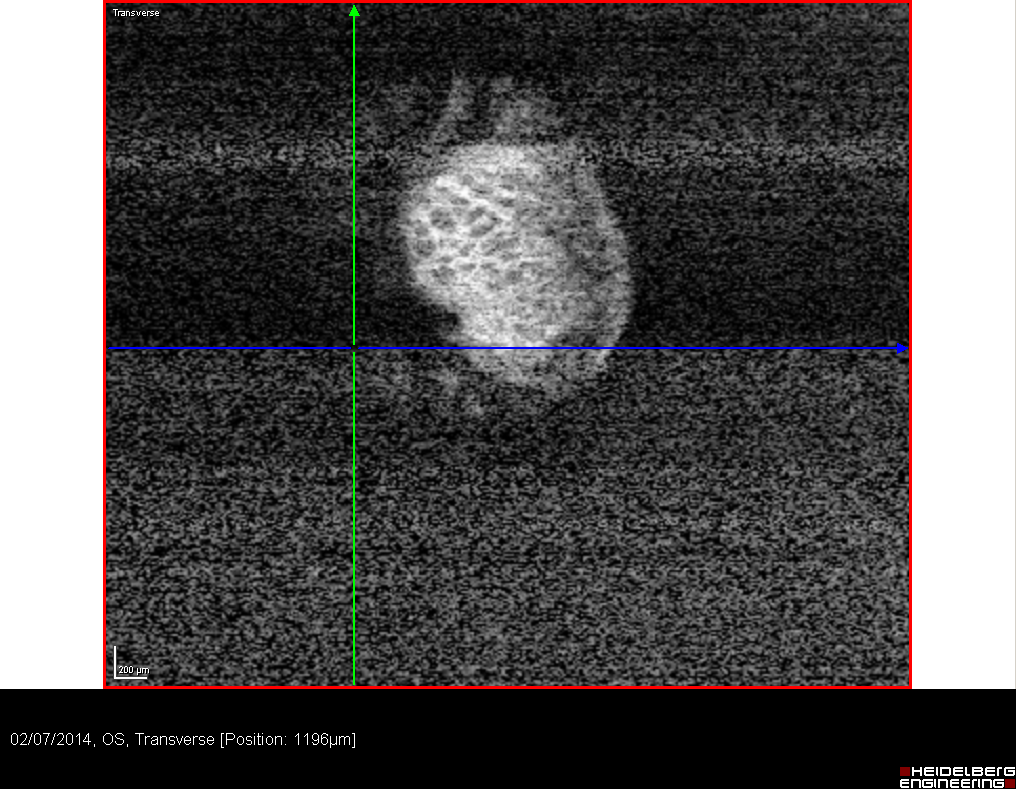
\includegraphics[width=\textwidth]{imagenes/conclusiones/PorosOriginal.png}}
    \end{figure}

Using the tradicional method the result is the following:

    \begin{figure}[H]
      \caption{Image given by medical staff}
      \centering \setlength\fboxsep{0pt} \setlength\fboxrule{0.5pt}
      \fbox{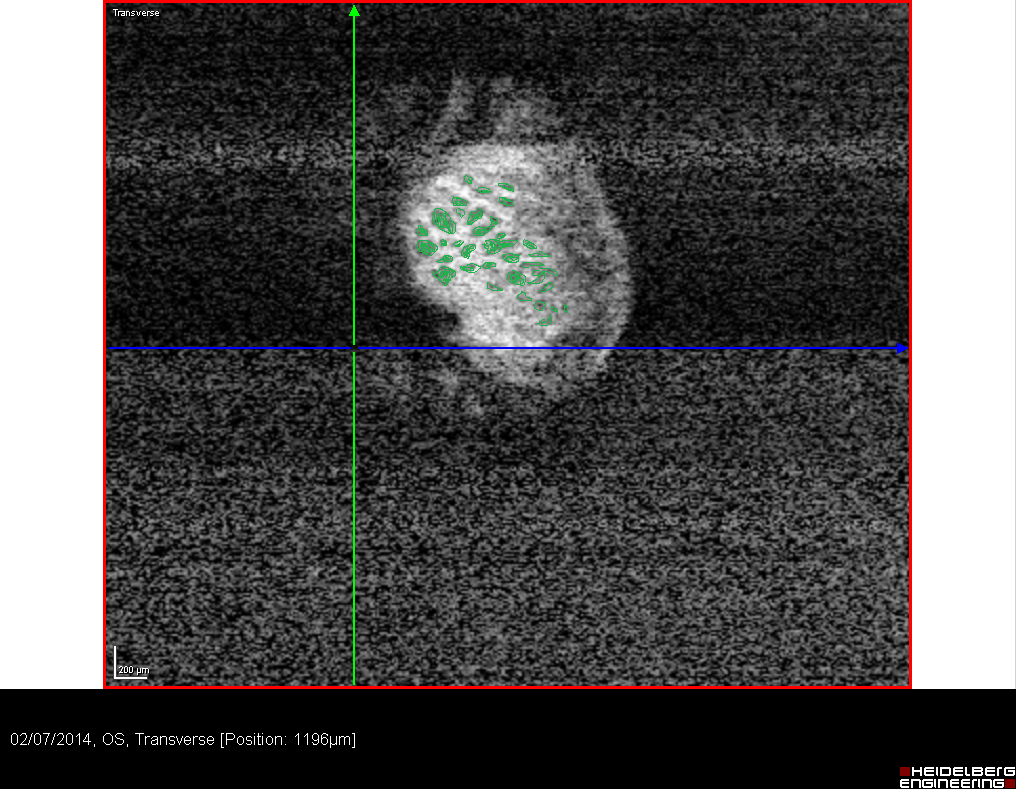
\includegraphics[width=\textwidth]{imagenes/conclusiones/PorosMedicos.png}}
    \end{figure}

Our algorithms can detect still more pores as it can be see in the next images.\\
OpenCV algorithm:

    \begin{figure}[H]
      \caption{OpenCV algorithm}
      \centering \setlength\fboxsep{0pt} \setlength\fboxrule{0.5pt}
      \fbox{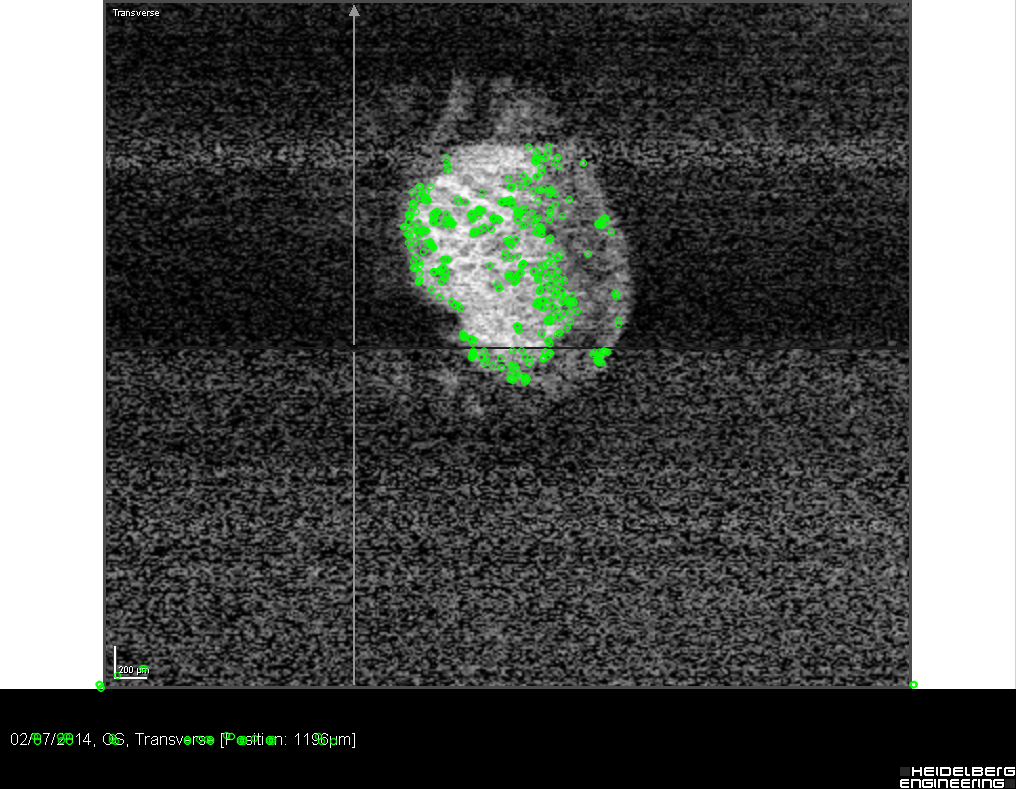
\includegraphics[width=\textwidth]{imagenes/conclusiones/PorosOpenCV.png}}
    \end{figure}

SimpleCV algorithm:

    \begin{figure}[H]
      \caption{SimpleCV algorithm}
      \centering \setlength\fboxsep{0pt} \setlength\fboxrule{0.5pt}
      \fbox{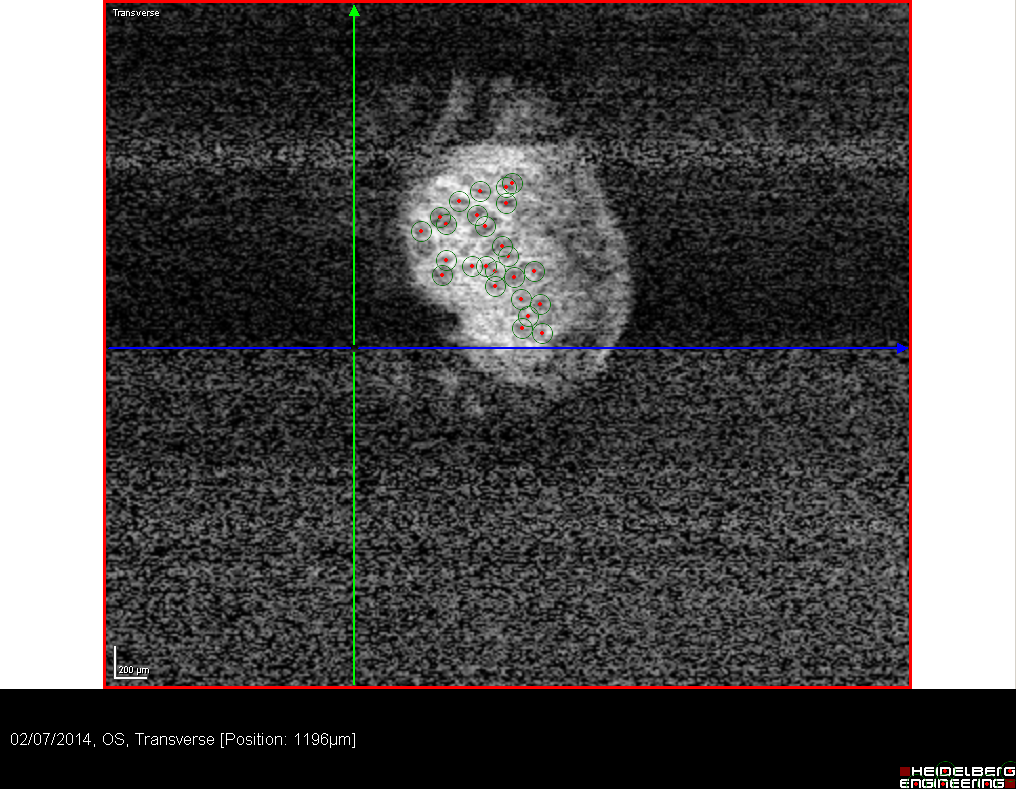
\includegraphics[width=\textwidth]{imagenes/conclusiones/PorosSimpleCV.png}}
    \end{figure}

The detection with these algorithms is faster and more reliable, and it
also provides the exact pores' size. This way it is no necessary to
stimate the ratio of the pores extension over the papilla surface.


\section{Conclusions about the measurement of the choroid thickness}
About the usage of Computer Vision algorithms for the measurement of
the \emph{choroid} thickness the results could not be better:
it has reached an exact precission in the measurement for the majority
of the images and imperceptible diferences on the worst cases, when
the noise or quality make harder the detection of the points.
Also the time of processing got reduced to less than a second without
the need of a doctor to do it. This does that the imprecissions
causes by human fails got removed, as we can see in the next example:

    \begin{figure}[H]
      \caption{Manually measurement}
      \centering \setlength\fboxsep{0pt} \setlength\fboxrule{0.5pt}
      \fbox{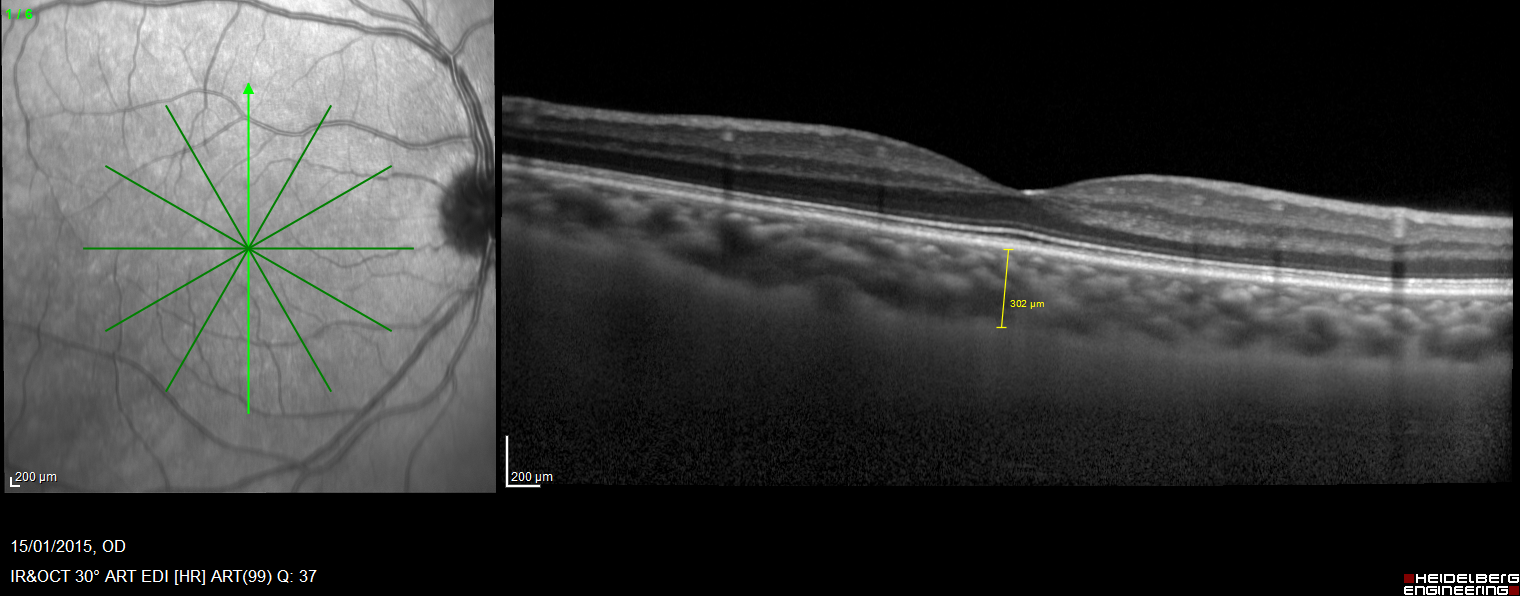
\includegraphics[width=\textwidth]{imagenes/conclusiones/EjemploConclusionMedicos.png}}
    \end{figure}

Using our algorithm and combining the images in order to compare them:

    \begin{figure}[H]
      \caption{Our algorithm measurement}
      \centering \setlength\fboxsep{0pt} \setlength\fboxrule{0.5pt}
      \fbox{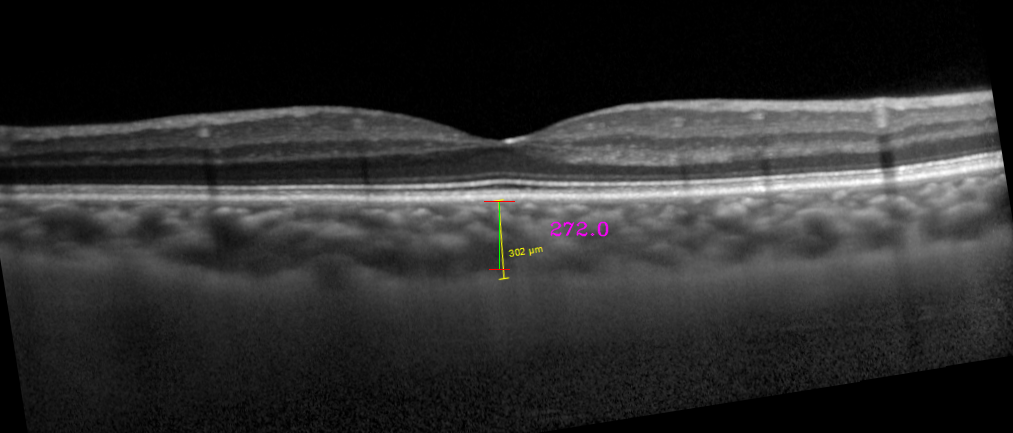
\includegraphics[width=\textwidth]{imagenes/conclusiones/EjemploConclusionCombinada.png}}
    \end{figure}

As we can see, the line manually traced (the yellow one) take a detour
to the right. The cause of this mistake is that it is so hard to the brain
to trace a perpendicular line when the image is spined. \\
Also the halo generated by the reflection of the light on the tissue
has been removed from the measurement due to prevent mistakes at the 
measurement time.
